\documentclass[border=0pt]{standalone}
\usepackage{fontspec}
\setmainfont{Liberation Serif}
\usepackage{unicode-math}
\setmathfont{latinmodern-math.otf}
\usepackage{tkz-euclide}
\usetikzlibrary{arrows.meta,calc,intersections,decorations.markings,angles,quotes}

% tkz-euclide assumes centimetre coordinates. Fonts and strokes use print sizes.
\tikzset{
  every picture/.style={x=1cm,y=1cm,line width=.55pt,line cap=round,line join=round,font=\fontsize{11}{13}\selectfont},
  every node/.style={inner sep=2pt},
  construction/.style={densely dashed,line width=.4pt},
  dimension/.style={<->,>=Stealth,line width=.4pt},
  vector/.style={postaction=decorate,decoration={markings,mark=at position .55 with {\arrow{Stealth[length=4pt,width=3pt]}}}},
  note/.style={font=\fontsize{9}{11}\selectfont\itshape,draw=black!65,line width=.35pt,inner sep=3pt,align=center},
  point/.style={circle,fill=black,inner sep=0pt,minimum size=1.8pt},
  axis/.style={-{Stealth[length=4pt,width=3pt]},line width=.45pt}
}
\newcommand{\NotToScale}[1]{\node[note] at #1 {Diagram is\\NOT to scale};}
% Fix the output canvas so Typst does not resize typography to fit label extents.
\newcommand{\ExamBounds}[2]{\pgfresetboundingbox\path[use as bounding box] (0,0) rectangle (#1mm,#2mm);}

\begin{document}
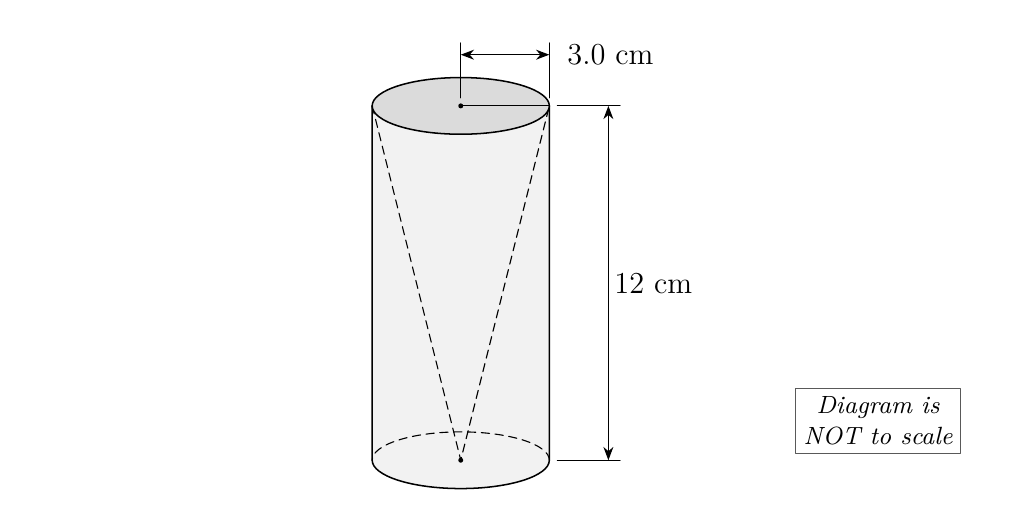
\begin{tikzpicture}
  % True proportions: r = 3.0 cm, h = 12 cm at 0.375 cm per cm (page coordinates in cm).
  % The cone is inserted apex down, so its base fills the canister's top.
  \def\R{1.125} \def\H{4.5} \def\ry{.36}
  \coordinate (T) at (5.5,5);
  \coordinate (Bc) at ($(T)+(0,-\H)$);
  \fill[black!5] ($(T)+(-\R,0)$) arc[start angle=180,end angle=360,x radius=\R,y radius=\ry] -- ($(Bc)+(\R,0)$) arc[start angle=0,end angle=-180,x radius=\R,y radius=\ry] -- cycle;
  % Hidden: back of the base rim and the cone's slant edges inside the canister.
  \draw[construction] ($(Bc)+(\R,0)$) arc[start angle=0,end angle=180,x radius=\R,y radius=\ry];
  \draw[construction] ($(T)+(-\R,0)$) -- (Bc) -- ($(T)+(\R,0)$);
  % Visible outline.
  \draw ($(T)+(-\R,0)$) -- ($(Bc)+(-\R,0)$) arc[start angle=180,end angle=360,x radius=\R,y radius=\ry] -- ($(T)+(\R,0)$);
  \filldraw[fill=black!14] (T) ellipse[x radius=\R,y radius=\ry];
  \draw[line width=.4pt] (T) -- ($(T)+(\R,0)$);
  \node[point] at (T) {};
  \node[point] at (Bc) {};
  % Radius dimension above the top, height dimension to the right.
  \draw[line width=.3pt] ($(T)+(0,.1)$) -- ($(T)+(0,.8)$) ($(T)+(\R,.1)$) -- ($(T)+(\R,.8)$);
  \draw[dimension] ($(T)+(0,.65)$) -- ($(T)+(\R,.65)$);
  \node[anchor=west] at ($(T)+(\R+.15,.65)$) {3.0 cm};
  \draw[line width=.3pt] ($(T)+(\R+.1,0)$) -- ($(T)+(\R+.9,0)$) ($(Bc)+(\R+.1,0)$) -- ($(Bc)+(\R+.9,0)$);
  \draw[dimension] ($(T)+(\R+.75,0)$) -- node[right] {12 cm} ($(Bc)+(\R+.75,0)$);
  \NotToScale{(10.8,1)}
  \ExamBounds{124}{59.9333}
\end{tikzpicture}
\end{document}
